\documentclass{standalone}
\usepackage{tikz, pgfplots, xcolor}
% \usepackage{pgfplots}
\begin{document}

\definecolor{eek}{RGB}{255,255,255}
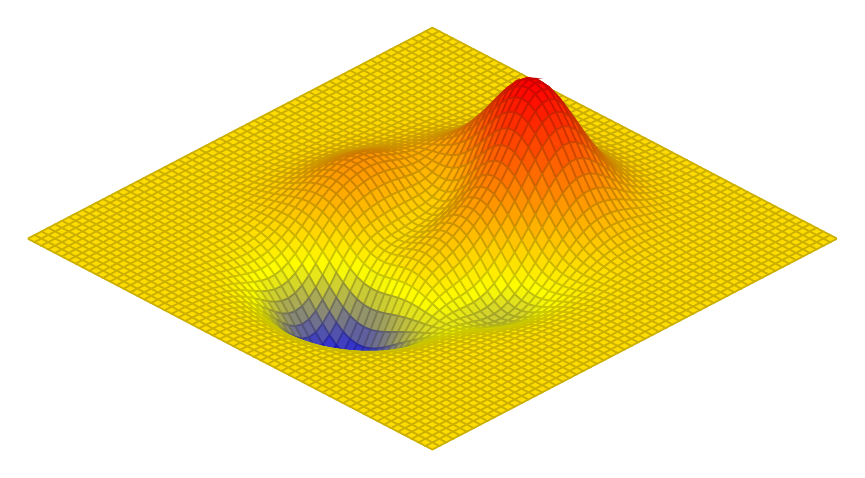
\begin{tikzpicture}[
  scale=1.5,
  declare function = {
    a(\x, \y) = 3*(1-\x)^2 * exp(-(\x^2)-(\y+1)^2);
    b(\x, \y) = -10*(\x/5 - \x^3 + \y^5) * exp(-\x^2 - \y^2);
    c(\x, \y) = -exp(-(\x+1)^2 - \y^2)/3;
    Z(\x, \y) = a(\x,\y) + b(\x,\y) + c(\x,\y);
  }
  ]
  \begin{axis}[
    view={225}{50},
    hide x axis,
    hide y axis,
    hide z axis,
    domain=-3.5:3.5,
    samples=60,
    ]
    \addplot3 [surf] {Z(x,y)};
  \end{axis}
\end{tikzpicture}
\end{document}
